%%%%%%%%%%%%%%%%%%%%%%%%%%%%%%%%%%%%%%%%%
% Journal Article
% LaTeX Template
% Version 1.4 (15/5/16)
%
% This template has been downloaded from:
% http://www.LaTeXTemplates.com
%
% Original author:
% Frits Wenneker (http://www.howtotex.com) with extensive modifications by
% Vel (vel@LaTeXTemplates.com)
%
% License:
% CC BY-NC-SA 3.0 (http://creativecommons.org/licenses/by-nc-sa/3.0/)
%
%%%%%%%%%%%%%%%%%%%%%%%%%%%%%%%%%%%%%%%%%

%----------------------------------------------------------------------------------------
%	PACKAGES AND OTHER DOCUMENT CONFIGURATIONS
%----------------------------------------------------------------------------------------

\documentclass[12pt]{article}
\usepackage[a4paper,headsep=0.6cm,left=2cm,right=2cm,top=2cm,bottom=2cm,twoside]{geometry}
\usepackage{graphics,graphicx}
\usepackage[utf8]{inputenc}
\usepackage[english,russian]{babel}
\usepackage[T2A]{fontenc}
\usepackage{amsmath,amssymb,amsthm,lomread}


\usepackage{microtype} % Slightly tweak font spacing for aesthetics

\usepackage[hmarginratio=1:1,top=32mm,columnsep=20pt]{geometry} % Document margins
\usepackage[hang, small,labelfont=bf,up,textfont=it,up]{caption} % Custom captions under/above floats in tables or figures
\usepackage{booktabs} % Horizontal rules in tables

\usepackage{lettrine} % The lettrine is the first enlarged letter at the beginning of the text

\usepackage{enumitem} % Customized lists
\setlist[itemize]{noitemsep} % Make itemize lists more compact

\usepackage{abstract} % Allows abstract customization
\renewcommand{\abstractnamefont}{\normalfont\bfseries} % Set the "Abstract" text to bold
\renewcommand{\abstracttextfont}{\normalfont\small\itshape} % Set the abstract itself to small italic text

\usepackage{titlesec} % Allows customization of titles
\renewcommand\thesection{\Roman{section}} % Roman numerals for the sections
\renewcommand\thesubsection{\roman{subsection}} % roman numerals for subsections
\titleformat{\section}[block]{\large\scshape\centering}{\thesection.}{1em}{} % Change the look of the section titles
\titleformat{\subsection}[block]{\large}{\thesubsection.}{1em}{} % Change the look of the section titles

\usepackage{fancyhdr} % Headers and footers
\pagestyle{fancy} % All pages have headers and footers
\fancyhead{} % Blank out the default header
\fancyfoot{} % Blank out the default footer
\fancyhead[C]{Валютные риски и монополизация майнинговой сети BTC $\bullet$ Сентябрь 2018} % Custom header text
\fancyfoot[RO,LE]{\thepage} % Custom footer text

\usepackage{titling} % Customizing the title section

\usepackage{hyperref} % For hyperlinks in the PDF


\usepackage{graphicx}
\graphicspath{ {./img/} }
\usepackage{float}
%----------------------------------------------------------------------------------------
%	TITLE SECTION
%----------------------------------------------------------------------------------------

\setlength{\droptitle}{-4\baselineskip} % Move the title up

\pretitle{\begin{center}\Huge\bfseries} % Article title formatting
\posttitle{\end{center}} % Article title closing formatting
\title{Оценка зависимости рисков трейдинга от степени монополизации вычислительных мощностей сети биткойн} % Article title
\author{%
\textsc{Егор Замотаев} \\[1ex] % Your name
\normalsize Алтайский государственный университет \\ % Your institution
\normalsize \href{mailto:egor.zamotaev@mail.ru}{egor.zamotaev@mail.ru} % Your email address
%\and % Uncomment if 2 authors are required, duplicate these 4 lines if more
%\textsc{Jane Smith}\thanks{Corresponding author} \\[1ex] % Second author's name
%\normalsize University of Utah \\ % Second author's institution
%\normalsize \href{mailto:jane@smith.com}{jane@smith.com} % Second author's email address
}
\date{\today} % Leave empty to omit a date
\renewcommand{\maketitlehookd}{%
\begin{abstract}
\noindent В данной статье рассматривается вопрос о влиянии степени монополизации майнинга криптовалюты биткойн на величину валютных рисков связанных с трейдингом данной криптовалюты на основных криптовалютных биржах. Для оценки степени монополизации используется индекс Херфиндаля-Хиршмана для хэшрейта основных майнинговых пулов BTC. На основе рассчёта коэффициента корреляции между данным индексом и величиной валютных рисков, полученных за текущий квартальный период, делается вывод о наличии существенной положительной связи между степенью монополизации майнинга биткойн и валютными рисками (чем больше монополизация, тем больше риски). Работа может быть полезна как для исследователей криптовалют, так и для криптовалютных трейдеров, а так же простым людям.
\end{abstract}
}

%----------------------------------------------------------------------------------------

\begin{document}

% Print the title
\maketitle

%----------------------------------------------------------------------------------------
%	ARTICLE CONTENTS
%----------------------------------------------------------------------------------------

\section{Ведение}

После событий 17 декабря 2017 года, когда цены на биткойн взлетели до уровня в 20000\$, в обществе возник неподдельный интерес к теме трейдинга на криптовалютных биржах. В общественных местах массово стали появляться объявления так или иначе связанные с криптовалютой биткойн, биржевым трейдингом, услугами повышения финансовой грамотности. Мотивация компаний предлагающих данные услуги совершенна ясна и не требует детального рассмотрения, в связи с чем нет оснований доверять подобным компаниям и предоставляемой ими информации. И в тоже время, для нас как учённых имеется потребность разобраться во всём происходящим в области криптовалют, понять истинные причины происходящего\footnote{В этом отношении очень хороши работы \cite{Malanov} и \cite{Dembinskaya}} на криптовалютных биржах, философски осмыслить значимость криптовалют в жизни нашего общества, оценить пользу и вред, которую может принести нам эта технология в будущем. Для этого должна быть проделана большая работа.
\par В данной статье рассматривается лишь малая её часть "--- исследование одной из закономерностей в области трейдинга на криптовалютных биржах, а именно "--- зависимость величины валютных рисков от степени монополизации для майнинговых пулов биткойн. Майнинг криптовалюты "--- процесс включающий в себя нахождение нового блока транзакций\footnote{Блокчейн-технология}, требующий определённых вычислительных мощностей\footnote{Для биткойн данный процесс в основном связан с вычислением хэш-значений по алгоритму SHA256} В нашем случае нас интересует то каким образом майнеру назначается вознаграждение. 
\par Вознаграждение назначается тому майнеру, который нашёл блок транзакций первым. Для поиска блока как правило требуется выполнить большое количество операций вычисления хэш-значений. В связи с этим для оценки вычислительных мощностей используют величину хэшрейта\footnote{hashrate}, выраженную в количестве операций подсчёта хэшей за единичный интервал времени\footnote{Т.е. за секунду (имеет размерность H/s)}. Поэтому вероятность того, что кто-либо из майнеров найдёт блок первым, тем выше, чем выше хэшрейт вычислительного ресурса, которым он распологает. На определённом этапе развития технологий майнинга\footnote{Использование дорогостоящих компьютерных видеокарт, а также специализированных микросхем для рассчёта хэш-функции, подстегнуло гонку добычи криптовалюты и единственным выходом для больших масс майнеров оказалось объединить свои компьютеры в распределённые сетевые кластеры для увеличения совместных вычислительных мощностей.} возникла потребность в объединении майнеров в т.н. майнинговые пулы, разделяющих между собой вознаграждения за найденные совместными усилиями блоки транзакций. Таким образом мы имеем множество майнинговых пулов, характеризуемых значениями хэшрейтов, что позволяет нам делать выводы о том, в какой степени монополизирована область майнинга криптовалюты, на основе вычисления индекса Херфиндаля-Хиршмана для хэшрейтов данной криптовалюты \footnote{В нашем случае это биткойн}.
\par В тоже время мы хотим понять насколько сильно монополизация вычислительных мощностей майнинговых пулов влияет на валютные риски трейдинга на криптовалютных биржах. 

%------------------------------------------------

\section{Методы}

В данной работе в качестве основного метода используется 
корреляционный анализ. Выдвигается альтернативная гипотеза $H_1$ о том, что между индексом Херфиндаля-Хиршмана для хэшрейтов основных биткойн пулов и величиной валютных рисков имеется некоторая (скорее всего положительная) связь. Основная гипотеза $H_0$ заключается в том, что данная связь отсутствует. 

\par Индекс Херфиндаля-Хиршмана вычисляется на основе имеющихся данных хэшрейтов накопленных за текущий квартальный период по формуле:

\begin{equation}
HHI =\sum_{i=1}^N s_i^2
\end{equation}
где $s_i$ "--- доля хэшрейта $i$-го пула, выраженная в процентах.

\par Для большей общности величина валютных рисков рассчитывается на основе данных по усреднённой стоимости криптовалюты биткойн для основных криптовалютных бирж (Kraken, Coinbase, Bitstamp, Itbit). Для вычислений используется формула:
\begin{equation}
VaR=u_{{\alpha }}\sigma _{r}-\mu _{r}
\end{equation}
Здесь \newline
$\mu _{r}$ "--- среднее значение темпа возможного прироста стоимости для биткойн \newline
$\sigma _{r}$ "--- дисперсия для тойже величины \newline
$u_{{\alpha }}$ "--- $\alpha$-квантиль стандартного нормального распределения

\par Далее для величин $HHI$ и $VaR$ вычисляется коэффициент корреляции Пирсмана:
\begin{equation} \label{eqn:r}
\mathbf {r}_{XY}={\frac {\mathbf {cov}_{XY}}{{\sigma}_{X}{\sigma}_{Y}}}={\frac {\sum (X-{\bar {X}})(Y-{\bar {Y}})}{\sqrt {\sum (X-{\bar {X}})^{2}\sum (Y-{\bar {Y}})^{2}}}}
\end{equation}
где 
$\overline {X}, \overline{Y}$ "--- средние значения выборок\footnote{Стоит отметить, что вычисленные данные по индексу Херфиндаля и валютным рискам представляют собой временные ряды, то есть коррелирование производится между двумя временными рядами. Подобный подход был применён в работе \cite{Kenneth}.}.

\par Для проверки основной гипотезы $H_0$ вычисляется P-значение, показывающее вероятность ошибки первого рода (вероятность того, что гипотеза неверно отвергнута при том, что она верна). Затем данная величина рассматривается как непрерывная и делается соответствующий статистический вывод о справедливости альтернативной гипотезы $H_1$.

%------------------------------------------------

\section{Результаты}

Рассчётные данные по зависимости валютных рисков от индекса Херфиндаля-Хиршмана представлены в таблице \ref{tab:thvar}:

\begin{table}[H]
\centering
\begin{tabular}{ccc}
\hline
Дата       & HHI  & VaR  \\ \hline
2018-03-19 & 1721 & 1487 \\
2018-03-26 & 1750 & 1235 \\
2018-04-02 & 1824 & 1160 \\
2018-04-09 & 1968 & 975  \\
2018-04-16 & 1967 & 687  \\
2018-04-23 & 2147 & 2538 \\
2018-04-30 & 1836 & 3629 \\
2018-05-07 & 2128 & 2663 \\
2018-05-14 & 2016 & 830  \\
2018-05-21 & 1878 & 779  \\
2018-05-28 & 1797 & 704  \\
2018-06-04 & 1925 & 781  \\
2018-06-11 & 2140 & 814  \\
2018-06-18 & 2015 & 708  \\
2018-06-25 & 1951 & 765  \\
2018-07-02 & 1981 & 460  \\
2018-07-09 & 1741 & 443  \\
2018-07-16 & 1830 & 687  \\
2018-07-23 & 1904 & 645  \\
2018-07-30 & 2234 & 761  \\
2018-08-06 & 2048 & 725  \\
2018-08-13 & 1971 & 765  \\
2018-08-20 & 1925 & 549  \\
2018-08-27 & 1968 & 406  \\ \hline
\end{tabular}
\caption{Динамика изменения индекса Херфиндаля-Хиршмана $HHI$ и величины валютных рисков $VaR$}
\label{tab:thvar}
\end{table}

Для большей наглядности вычисленные значения отображены на графике \ref{img:varh}:

\begin{figure}[H]
\centering
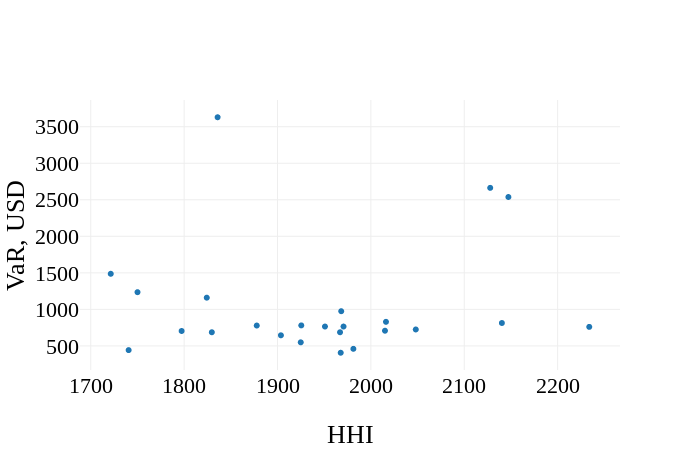
\includegraphics[width=0.5\textwidth]{varh.png}
\caption{Пары значений валютных рисков $VaR$ и величин индекса Херфиндаля-Хиршмана $HHI$ отнесённые к одинаковым временным интервалам}
\label{img:varh}
\end{figure}

Как видно из графика \ref{img:varh} часть данных не вписываются в общую картину, что может быть связано с воздействием каких-либо сторонних факторов, повлиявших на величину $VaR$\footnote{Примечание: Данные на графике \ref{img:varh} в правом верхнем углу расположены очень близко по времени и скорее всего относятся к одному и тому же ряду событий (апрель-май 2018-го)}. Для устранения данных возможного влияния посторонних факторов была произведена предварительная фильтрация, после которой данные приобрели вид:

\begin{figure}[H]
\centering
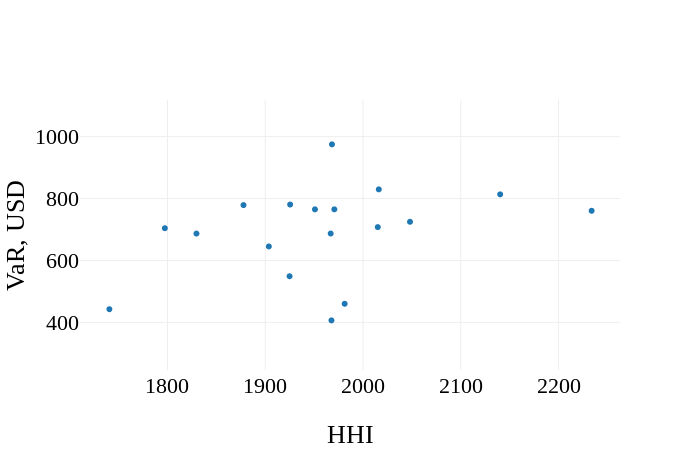
\includegraphics[width=0.5\textwidth]{varh_filtered.png}
\caption{Пары значений валютных рисков $VaR$ и величин индекса Херфиндаля-Хиршмана $HHI$ после фильтрации}
\label{img:varhf}
\end{figure}
На графике видно, что между $VaR$ и $HHI$ имеется некоторая положительная связь. Для оценки величины данной связи по формуле (\ref{eqn:r}) был вычислен коэффициент корреляции Пирсмана\footnote{Данный коэффициент был посчитан для данных накопленных за текущий квартальный период (3 месяца)}, который составил 0.48 при P-значении равном 0.09. В первом приближении это значит, что с вероятностью в 91\% действительный коэффициент корреляции между величинами $VaR$ и $HHI$ имеет величину не менее 0.48. 
\par Исходя из этого, а так же учитывая представленную выше информацию, можно сделать вывод о том, что степень монополизации области майнинговых пулов существенно влияет на величину валютного риска (чем больше монополизация, тем больше риски). Таким образом принимается альтернативная гипотеза $H_1$.
\par Данный вывод естественным образом вписывается в текущее понимание ситуации торговли биткойнами на криптовалютных биржах, отражая тот факт, что состояние бирж определяется как правило крупными финасовыми игроками, относящимися к наиболее крупным майнинговым пулам, по-преимуществу владеющими большей частью вычислительных ресурсов сети биткойн.
%------------------------------------------------

\section{Обсуждение}

\subsection{Вопрос первый}

Какой в действительности явялется форма связи между $VaR$ и $HHI$, является ли она линейной?

\par Если внимательно посмотреть на график \ref{img:varhf}, то можно увидеть, что форма зависимости между $VaR$ и $HHI$ скорее всего нелинейная "--- с ростом величины $HHI$ величина $VaR$ растёт всё медленнее "--- это вполне возможно. К сожалению неизвестно как влияют на величину $VaR$ другие факторы. Для проведения более детального исследования необходимо рассмотрение всего множества иных факторов, могущих влиять на данную величину. Для этого хорошо воспользоваться, к примеру, дисперсионным анализом.

\subsection{Вопрос второй}
С чем связаны значительные выбросы на графике?
\par Возможно, что значительные колебания в $VaR$ значении на начало года были вызваны ажиотажем искусственно созданным вокруг торговли биткойнами на криптовалютных биржах\cite{Dembinskaya}. Для выяснения истинной причины требуется выйти за рамки данной работы и провести анализ общего информационного фона сложившегося вокруг биткойн валюты за значительный период времени, начиная с событий предшествоваших резкому скачку стоимости от 17 декабря 2017 года.
%----------------------------------------------------------------------------------------
%	REFERENCE LIST
%----------------------------------------------------------------------------------------
 \bibliographystyle{gost1}
 \bibliography{Articles,Internet}

%----------------------------------------------------------------------------------------

\end{document}
